\chapter{ОРГАНИЗАЦИОННО-ЭКОНОМИЧЕСКАЯ ЧАСТЬ}
\label{cha:ch_5}

В данной работе рассматривается создание противотанкового комплекса, включающего в себя противотанковую управляемую ракету (ПТУР), на основе беспилотного летательного аппарата. В рамках работ по проекту проводится исследование различных методов наведения ПТУР для получения заданной траектории и проработка конструкции ГСН. Эти работы вынесены в отдельный НИР.

НИР проводится на кафедре СМ6 в МГТУ им. Баумана. По данной теме задействовано два исполнителя: исследователь и инженер. Срок выполнения работы: два года.

Ранее аналогичные по объему и принципу исследования работы на кафедре СМ6 не производились.

Задачи организационно-экономической части:
\begin{enumerate}[1.]
	\item Разработка план-графика выполнения НИР;
	\item Расчет сметы затрат на выполнение НИР;
\end{enumerate}

\clearpage
\section{Формирование структуры НИР}
Состав НИР по созданию комплекса и исполнители каждого этапа представлены в таблице \ref{tab:econ_nir_struct}.
\begin{table}[h]
	\begin{center}
		\caption{Состав проводимого НИР}
		\begin{tabular}{|p{8mm}|p{30mm}|p{70mm}|p{40mm}|}
  		\hline
№ & Этап НИР & Содержание работ & Исполнитель \\ \hline
1 & Техническое задание (ТЗ) & Постановка задачи. Формирование исходных данных. & Исследователь \\ \hline
2 & Эскизный проект (ЭП) & Формирование списка вариантов закона наведения и устройства ГСН. & Инженер, исследователь \\ \hline
3 & Технический проект (ТП) & Детальная проработка выбранного варианта. Проведение моделирования. & Инженер, исследователь \\ \hline
4 & Рабочий проект (РП) & Разработка рабочих чертежей, корректировка расчетов. & Инженер, исследователь \\ \hline
5 & Внедрение & Анализ полученных результатов. Формирование отчета. & Исследователь \\ \hline
		\end{tabular}
		\label{tab:econ_nir_struct}
	\end{center}
\end{table}

\clearpage
\section{Определение трудоемкости этапов НИР}
Трудоемкость этапа можно определить одним из следующих методов:
\begin{itemize}
	\item методом вероятностных оценок;
	\item методом экспертного опроса;
	\item методом аналогии;
	\item методом прямого нормирования (на базе существующих нормативов).
\end{itemize}

Метод вероятностных оценок применяется для оценки длительности работ, а также для оценки трудоемкости. Суть метода в том, что непосредственный руководитель работ, имеющий опыт по их проведению и располагающий определенным составом исполнителей, оценивает максимальную и минимальную трудоемкости выполнения работ по этапам.

При методе экспертного определения трудоемкости эту величину оценивает не один специалист, а несколько, что позволяет уменьшить ошибки при планировании. При этом каждый эксперт может использовать изложенную выше систему вероятностных оценок.

Метод аналогии часто применяется для определения трудоемкости выполнения отдельных этапов работ, основанный на использовании накопленного статистического материала по трудоемкости ранее выполненных работ с учетом поправочных коэффициентов.

Метод прямого нормирования при расчете трудоемкости этапов НИР может быть использован только частично, как правило, для таких работ, как чертежно-графические, копировальные, работы по проектированию моделей или стенда, проведения эксперимента.

Так как при выполнении данной работы надежные источники норм времени отсутствуют, рекомендуется использовать экспертный метод определения трудоемкости работы при установленном количестве исполнителей. В качестве эксперта выступает ответственный исполнитель, принимавший участие в проведении данной НИР. Результаты оценки рассматриваются не как обязательство ответственного исполнителя, а как предложение, основанное на опыте и на учете факторов, влияющих на продолжительность работы.

В данной работе использована двухточечная система оценки трудоемкости. Для каждого этапа в данном случае определяется минимальная $\tau_{min}$ и максимальная $\tau_{max}$  трудоемкость работы, соответственно отражающие наиболее благоприятное стечение обстоятельств и наименее благоприятное.

Ожидаемая трудоемкость исполнения каждого этапа работ определяется по формуле (\ref{form:econ_trud}).
\begin{equation}
	\tau_\text{ож} = \frac{3 \cdot \tau_{min} + 2 \cdot \tau_{max}}{5}
	\label{form:econ_trud}
\end{equation}

Минимальные и максимальные трудоемкости назначены руководителем проекта.

В таблице \ref{tab:econ_nir_trud} представлены величины трудоемкости каждого этапа НИР.
\begin{table}[h]
	\begin{center}
		\caption{Трудоемкость этапов НИР}
		\begin{tabular}{|p{6mm}|p{50mm}|p{29mm}|p{29mm}|p{29mm}|}
  		\hline
№ & Этапы НИР &  $\tau_{min}$, чел-дни &  $\tau_{max}$, чел-дни & $\tau_\text{ож}$, чел-дни \\ \hline
1 & Техническое задание (ТЗ) & 40 & 55 & 46 \\ \hline
2 & Эскизный проект (ЭП) & 350 & 380 & 362 \\ \hline
3 & Технический проект (ТП) & 250 & 350 & 290 \\ \hline
4 & Рабочий проект (РП) & 130 & 160 & 142 \\ \hline
5 & Внедрение & 45 & 70 & 55 \\ \hline
\multicolumn{2}{|p{55mm}|}{\textbf{Итого:}} & \textbf{815} & \textbf{1015} & \textbf{895} \\\hline
		\end{tabular}
		\label{tab:econ_nir_trud}
	\end{center}
\end{table}

\clearpage
\section{Разработка план-графика выполнения НИР}
Для составления план-графика необходимо знать длительность выполнения каждого этапа НИР. Длительность этапов в рабочих днях определяется по формуле \ref{form:time_in_chd}.
\begin{equation}
	T_\text{раб i} = \frac{ \tau_i } { R_i \cdot K_\text{вн} }
	\label{form:time_in_chd}
\end{equation}
Здесь $\tau_i$ - трудоемкость выполнения i-го этапа работы, чел-дни; $R_i$ - число исполнителей i-го этапа, чел-дни; $K_\text{вн}$ - коэффициент выполнения норм. Принимаем $K_\text{вн}$ = 1.

Длительность этапов в календарных днях определяется по формуле \ref{form:time_in_cal}:
\begin{equation}
	T_\text{K i} = T_\text{раб i} \cdot k_\text{р-х}
	\label{form:time_in_cal}
\end{equation}
Здаесь $k_\text{р-х}$ - коэффициент перевода рабочих дней в календарные. Исходя из среднегодового количества рабочих, выходных и праздничных дней в году $k_\text{р-х}$ можно принять равным 1,45.

Результат расчета длительности этапов НИР приведен в таблице \ref{tab:etaps_time_result}.
\begin{table}[h]
	\begin{center}
		\caption{Длительность этапов НИР}
		\begin{tabular}{|p{6mm}|p{29mm}|p{29mm}|p{29mm}|p{29mm}|}
		\hline
№ & T, чел-дни. & R, человек & $T_\text{раб}$ , дни & $T_K$, дни \\ \hline
1 & 46 & 1 & 46 & 67 \\ \hline
2 & 362 & 2 & 181 & 263 \\ \hline
3 & 290 & 2 & 145 & 211 \\ \hline
4 & 142 & 2 & 71 & 103 \\ \hline
5 & 55 & 1 & 55 & 80 \\ \hline
		\end{tabular}
		\label{tab:etaps_time_result}
	\end{center}
\end{table}

\clearpage
На основании рассчитанной продолжительности этапов строится календарный график выполнения НИР, изображенный на рисунке \ref{fig:econ_plan_graph}.

\begin{figure}[h]
	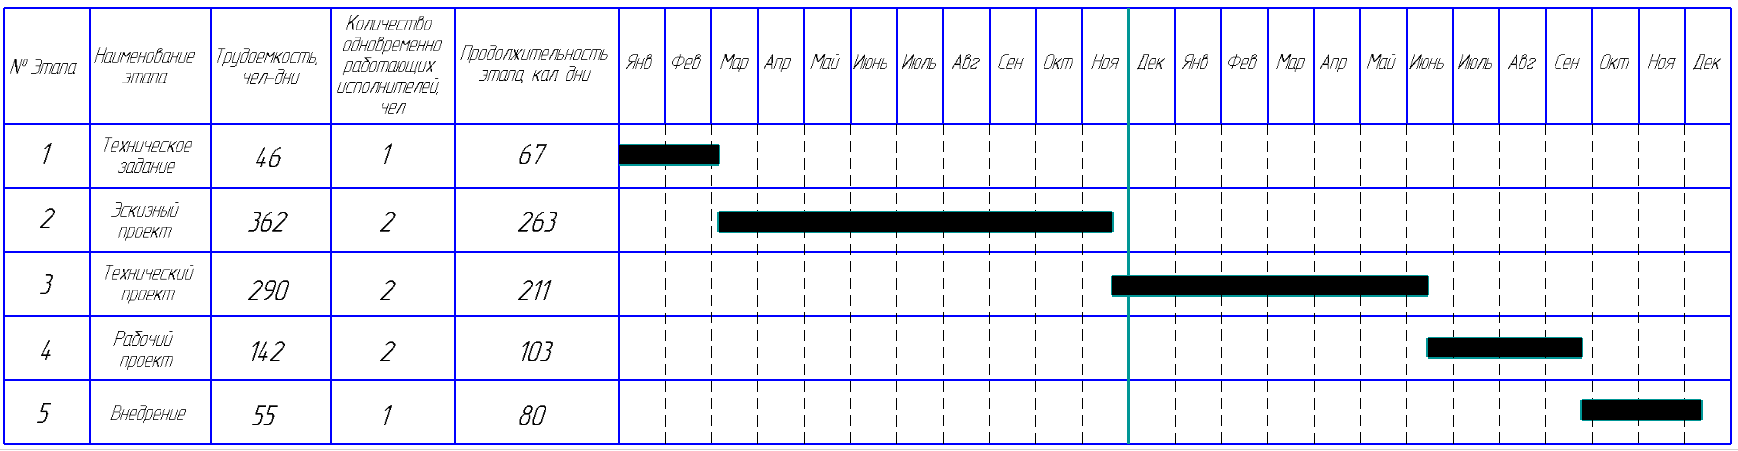
\includegraphics[width=\linewidth]{econ_plan_graph}
	\caption{План-график выполнения НИР}
	\label{fig:econ_plan_graph}
\end{figure}

Предварительная оценка работ по НИР показывает, что общее время работ составляет 1 год и 11 месяцев.

\clearpage
\section{Расчёт сметы затрат на НИР}
Смета затрат по тематике (калькуляция) является общей суммой расходов на проведение НИР в МГТУ им. Баумана.
Состав затрат, включаемых в смету на проведение НИР, определяется исходя из задач технического задания на проведение работы.
\begin{itemize}
	\item затраты на заработную плату работникам, непосредственно занятым при выполнении НИР (статья <<Заработная плата>> Сметы затрат);
	\item отчисления в фонды социального назначения (статья <<Отчисления в фонды социального назначения>>  Сметы затрат);
	\item материальные затраты (статья <<Материалы>> Сметы затрат);
	\item накладные расходы (статья <<Накладные расходы>> Сметы затрат).
\end{itemize}

\subsection{Статья <<Заработная плата>>}

На статью <<Заработная плата>> относятся выплаты работникам предприятия, непосредственно занятым выполнением НИР, а также выплаты лицам, не со¬стоящим в штате предприятия, по договорам гражданско-правового характера (в т.ч. по договорам подряда), относящимся к выполнению работы.

Объем фонда заработной платы определяется исходя из следующих данных:
\begin{itemize}
\item общее число работников, выполняющих НИР, в т.ч. по категориям персонала (руководитель проекта (фирмы), научные работники, инженерно-технические работники, бухгалтер, пр.);
\item должностные оклады в соответствии со штатным расписанием или приказом о выполнении НИР (при расчете следует руководствоваться принятыми в бюджетной сфере формами и системами оплаты труда с учетом отраслевой системы оплаты труда, принятой и утверждённой в отрасли);
\item количество месяцев выполнения НИР.
\end{itemize}

Должностные оклады для исполнителей, задействованных в НИР, приведены в таблице \ref{tab:econ_grades}.
\begin{table}[h]
	\begin{center}
		\caption{Оклады персонала}
		\begin{tabular}{|l|l|l|}
		\hline
№ & Должность исполнителя & Должностной оклад, руб. \\ \hline
1 & Исследователь & 42000 \\ \hline
2 & Инженер & 30000 \\ \hline
		\end{tabular}
		\label{tab:econ_grades}
	\end{center}
\end{table}

Дневные ставки исполнителей определим по формуле: $$C=\dfrac{Q_\text{п}\cdot12}{250},$$ где
$Q_\text{п}$ - месячный оклад исполнителя;
12 – число месяцев в году;
250 – приблизительное число рабочих дней в году.

Дневные ставки исполнителей (при 8-ми часовом рабочем дне): 
\begin{itemize}
	\item $C_\text{и}$=2016 руб/день– исследователя;
	\item $С_\text{р}$=1440 руб/день – инженера.
\end{itemize}

Заработная плата исполнителей по этапам работы приведена в таблице \ref{tab:eocn_grades_etap}.

\begin{table}[h]
	\begin{center}
		\caption{Заработная плата исполнителей по этапам}
		\begin{tabular}{|l|l|l|l|}
		\hline
Этап & Исполнитель & Занятость, раб. дни. & Заработная плата, руб \\ \hline
1 & Исследователь & 45 & 90720 \\ \hline
2 & Исследователь & 181 & 364896 \\ \cline{2-4}
 & Инженер & 181 & 260640 \\ \hline
3 & Исследователь & 145 & 392320 \\ \cline{2-4}
 & Инженер & 145 & 208800 \\ \hline
4 & Исследователь & 71 & 143136 \\ \cline{2-4}
 & Инженер & 71 & 102240 \\ \hline
5 & Исследователь & 55 & 110880 \\ \hline
 \multicolumn{3}{|p{100mm}|}{\textbf{Заработная плата $\sum $ ЗП} } & \textbf{1573632} \\
 \hline
		\end{tabular}
		\label{tab:eocn_grades_etap}
	\end{center}
\end{table}


\subsection{Статья <<Дополнительная заработная плата>>}
При выполнении работ по НИР возможно отклонение условий труда сотрудников от нормальных условий труда, предусмотренных Трудовым кодексом РФ. Также возможны выплаты сотрудникам, связанные с обеспечением гарантий и компенсаций – при исполнении государственных или общественных обязанностей, при совмещении работы с обучением, при предоставлении ежегодного оплачиваемого отпуска и т.д.

Размер дополнительных выплат характеризуется коэффициентом $\alpha$, выражающим отношение суммарных доплат к фонду основной оплаты персонала. В данном исследовании $\alpha$ принимается равным 0.15. Таким образом: $$\text{Доп. ЗП} = \sum \text{ЗП} \cdot 0.15 = 1573632 \cdot 0.15 = 236044 \text{ руб.} $$

\subsection{Статья <<Отчисления в фонды>>}
На статью <<Отчисления в фонды>> относятся расходы по уплате единого социального налога, начисляемого работодателем в соответствии с законодательством Российской Фе¬дерации, и взносов по страховым тарифам на обязательное социальное страхова¬ние от несчастных случаев на производстве и профессиональных заболеваний в соответствии с законодательством Российской Федерации. Начисления на заработную плату принимаются 30\% от ЗП (основной и дополнительной), эта сумма складывается из:
\begin{itemize}
	\item 22.0\% - отчисления в Пенсионный фонд;
	\item 2.9\% - отчисления в Фонд социального страхования;
	\item 5.1\% - отчисления в Федеральный фонд обязательного медицинского страхования.
\end{itemize}
$$\text{Отчисления} = \sum \text{ЗП + Доп. ЗП} \cdot 0.30 = (1573632+236044) \cdot 0.30 = 524903 \text{ руб.} $$

\subsection{Статья <<Материалы>>}
Затраты на материалы связаны с обеспечением рабочего места необходимым для ведения научной деятельности оборудованием и ПО. Перечень материалов приведен в таблице \ref{tab:econ_materials}.

\begin{table}[h]
	\begin{center}
		\caption{Затраты на материалы}
		\begin{tabular}{|l|l|l|l|l|}
		\hline
№ & Наименование & Цена, руб. & Количество & Сумма, руб. \\ \hline
1 & Бумага & 200 & 4 пачки & 800 \\ \hline
2 & Картриджи & 1000 & 2 шт. & 2000 \\ \hline
3 & Книги & 250 & 5 шт. & 1250 \\ \hline
 \multicolumn{4}{|p{100mm}|}{\textbf{ИТОГО}} & \textbf{1573632} \\
 \hline
		\end{tabular}
		\label{tab:econ_materials}
	\end{center}
\end{table}

Прочие затраты принимаются в размере 5\% от суммы основных затрат на материалы: $$\text{Общие затраты на материалы} = 1,05 \cdot M_\text{осн} = 1,05 \cdot 4250=4463 \text{ руб.} $$

\subsection{Статья <<Накладные расходы>>}
Накладные расходы включают расходы на производство, управление и хозяйственное обслуживание. Их величина вычисляется в процентах к основной заработной плате исполнителей. Для НИР в данном случае данная статья расходов принимается в размере 60\% от ЗП: $$ \text{Накладные расходы} = 0,60 \cdot \sum \text{ЗП} = 0,60 \cdot 1573632= 944180 \text{ руб}. $$

\clearpage
\section{Смета затрат на НИР}
Итоговая смета затрат на НИР приведена в таблице \ref{tab:econ_result}.

\begin{table}[h]
	\begin{center}
		\caption{Смета затрат на НИР}
		\begin{tabular}{|l|l|l|}
		\hline
Статья & Доля от общей суммы, \% & Затраты, руб. \\ \hline
Заработная плата & 47,93 & 1573632 \\ \hline
Дополнительная ЗП & 7,19 & 236045 \\ \hline
Отчисления в фонды & 15,99 & 524903 \\ \hline
Материалы & 0.14 & 4463 \\ \hline
Накладные расходы & 28,76 & 944180 \\ \hline
 \multicolumn{2}{|p{80mm}|}{\textbf{ИТОГО}} & \textbf{3283223} \\
 \hline
		\end{tabular}
		\label{tab:econ_result}
	\end{center}
\end{table}

